\begin{figure}
    \centering
    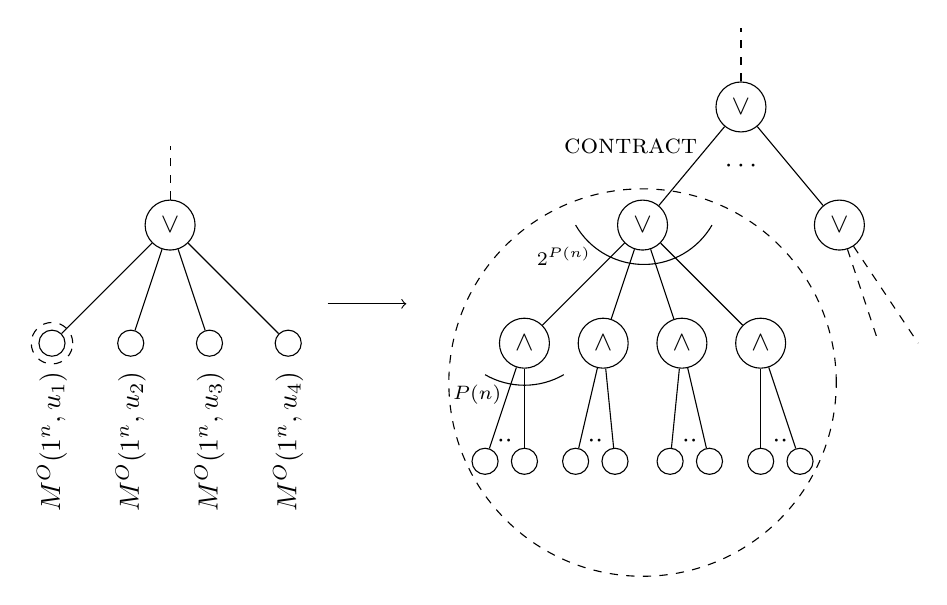
\begin{tikzpicture}

        % Circuit $C_n$
        \node[circle,draw] (parent) at (-3,0) {$\lor$};
        \node[circle,draw] (child1) at (-4.5,-1.5) {};
        \node[circle,draw] (child2) at (-3.5,-1.5) {};
        \node[circle,draw] (child3) at (-2.5,-1.5) {};
        \node[circle,draw] (child4) at (-1.5,-1.5) {};

        \node[rotate=90] (child1-label) at (-4.5, -2.75) {$M^{O}(1^n, u_1)$};
        \node[rotate=90] (child2-label) at (-3.5, -2.75) {$M^{O}(1^n, u_2)$};
        \node[rotate=90] (child3-label) at (-2.5, -2.75) {$M^{O}(1^n, u_3)$};
        \node[rotate=90] (child4-label) at (-1.5, -2.75) {$M^{O}(1^n, u_4)$};

        \draw [-] (parent) -- (child1);
        \draw [-] (parent) -- (child2);
        \draw [-] (parent) -- (child3);
        \draw [-] (parent) -- (child4);
        \draw [dashed] (parent) -- (-3,1);

        \node[draw,circle,dashed,minimum size=15pt] (OldCircuit) at (-4.5,-1.5) {};

        % The arrow
        \draw [->] (-1,-1) -- (0,-1);

        % Circuit $C'_n$
        \node [circle,draw] (grandparent) at (4.25,1.5) {$\lor$};

        \node [circle, draw] (absenteeparent) at (5.5,0) {$\lor$};
        
        \node[circle,draw] (parent) at (3,0) {$\lor$};
        \node[circle,draw] (child1) at (1.5,-1.5) {$\land$};
        \node[circle,draw] (child2) at (2.5,-1.5) {$\land$};
        \node[circle,draw] (child3) at (3.5,-1.5) {$\land$};
        \node[circle,draw] (child4) at (4.5,-1.5) {$\land$};

        \node[circle,draw] (grandchild11) at (1,-3) {};
        \node (grandchild1-dots) at (1.25,-2.75) {$\cdot \cdot$};
        \node[circle,draw] (grandchild12) at (1.5,-3) {};

        \node[circle,draw] (grandchild21) at (2.15,-3) {};
        \node (grandchild2-dots) at (2.4,-2.75) {$\cdot \cdot$};
        \node[circle,draw] (grandchild22) at (2.65,-3) {};

        \node[circle,draw] (grandchild31) at (3.35,-3) {};
        \node (grandchild2-dots) at (3.6,-2.75) {$\cdot \cdot$};
        \node[circle,draw] (grandchild32) at (3.85,-3) {};

        \node[circle,draw] (grandchild41) at (4.5,-3) {};
        \node (grandchild4-dots) at (4.75,-2.75) {$\cdot \cdot$};
        \node[circle,draw] (grandchild42) at (5,-3) {};
       
        \node[draw,circle,dashed,minimum size=140pt] (DNFpartInNewCircuit) at (3,-2) {};
    
        \draw [-] (grandparent) -- (parent);
        \draw [-] (grandparent) -- (absenteeparent);
        \draw [-] (parent) -- (child1);
        \draw [-] (parent) -- (child2);
        \draw [-] (parent) -- (child3);
        \draw [-] (parent) -- (child4);
        \draw [-] (child1) -- (grandchild11);
        \draw [-] (child1) -- (grandchild12);
        \draw [-] (child2) -- (grandchild21);
        \draw [-] (child2) -- (grandchild22);
        \draw [-] (child3) -- (grandchild31);
        \draw [-] (child3) -- (grandchild32);
        \draw [-] (child4) -- (grandchild41);
        \draw [-] (child4) -- (grandchild42);

        % Arc for exponential fan-in
        \draw[black] (2.15,0) arc (-150:-30:1);
        \node (exponential) at (2,-0.4) {\scriptsize $2^{P(n)}$};

        % Arc for polynomial fan-in
        \draw[black] (1,-1.9) arc (-120:-60:1);
        \node (poly) at (0.9,-2.15) {\scriptsize $P(n)$};

        \draw [dashed] (absenteeparent) -- (6,-1.5);
        \draw [dashed] (absenteeparent) -- (6.5,-1.5);
        \node [rotate=0] (dots) at (4.25,0.75) {$\cdots$};
        \draw [dashed] (grandparent) -- (4.25,2.5);
        \node [rotate=0] (Contract) at (2.85,1) {$\textsc{contract}$};

    \end{tikzpicture}
    \caption{Illustration of the circuit construction mentioned in the proof of \Cref{thm:CircuitLowerBoundsImplyNoMembershipInRPH}. In the first step of construction, each input node in the old circuit gets replaced by depth-$2$ circuits which have a fan-in of at most $P(n)$ for the gates that are the parents of the input nodes and have a fan-in of at most $2^{P(n)}$ for the gates that are the grandparents of the input nodes; here $P(n)$ is a polynomial. Furthermore, its input nodes are outputs of $M'^{O}$. The second step of the construction is to contract consecutive edges with the same labels. The final depth of the new circuit is $1$ more than the depth of the original circuit.}
    \label{fig:MachineMakesOneQuery}
\end{figure}